\documentclass[dvipdfmx]{jreport}
\usepackage{mypackage}
%%%%%%%%%%%%%%%%%%%%%%%%%%%%%%%%%%
\begin{document}

\chapter{原理}

\section{ニュートリノヘリシティの測定原理}
ニュートリノヘリシティの測定のために、$\ce{^{152\mathrm{m}}Eu}$の電子捕獲によるニュートリノを利用する。
\begin{equation}
  \label{EC}
  \ce{^{152\mathrm{m}}Eu} + \ce{e^{-}} \rightarrow \ce{^{152}Sm^{*}} + \nu_{e}
\end{equation}
ここで$\ce{^{152\mathrm{m}}Eu}$の半減期は$9.3\mathrm{h}$である。サマリウムの励起された原子核はガンマ線を出して基底状態に落ち着く。
\begin{equation}
  \label{gamma_emit}
  \ce{^{152}Sm^{*}} \rightarrow \ce{^{152}Sm} + \gamma
\end{equation}
この$\ref{gamma_emit}$で出たガンマ線のヘリシティを測定することで、ニュートリノのヘリシティを間接的に測定する。
ニュートリノと電子が共にスピン$\frac{1}{2}$の粒子であることから図$\ref{helicity_structure}$のように、
$\ce{Sm^{*}}$の前方に放出された$\gamma_{\mathrm{forward}}$がニュートリノのヘリシティを引き継いでいる。すなわち
\begin{equation}
  \label{helicity}
  h_{\nu} = h_{\gamma}
\end{equation}
である。
\begin{figure}[htbp]
  \begin{center}
    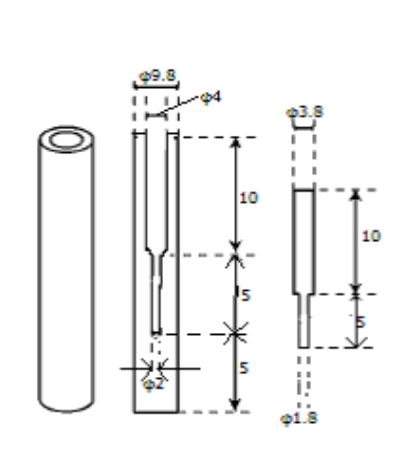
\includegraphics[width=50mm]{figure/case.png}
    \caption{$\ce{Eu}$の放射化の際に用いるケース \label{case}}
  \end{center}
\end{figure}
\begin{figure}[htbp]
  \begin{center}
    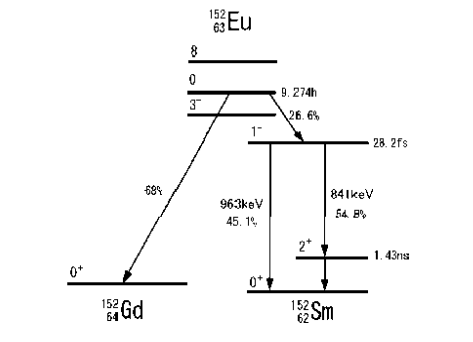
\includegraphics[width=100mm]{figure/decay_chain.png}
    \caption{$\ce{^{152\mathrm{m}}Eu}$の崩壊図式}
  \end{center}
\end{figure}
\begin{figure}[htbp]
  \begin{center}
    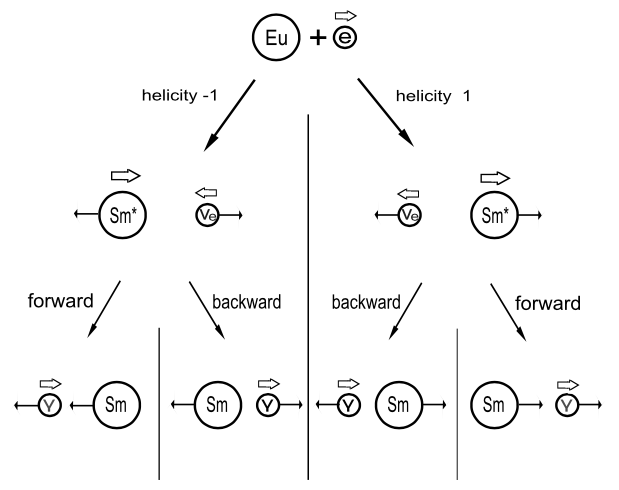
\includegraphics[width=100mm]{figure/helicity_structure.png}
    \caption{$\ce{^{152\mathrm{m}}Eu}$の崩壊 \label{helicity_structure}}
  \end{center}
\end{figure}

\section{ニュートリノヘリシティの測定手法}

\subsection{観測量からのニュートリノヘリシティの算出}
本実験でニュートリノヘリシティーを算出するのに用いる量は以下の通りである。
\begin{itemize}
\item $N_{+}$:ヘリシティーが$+$の$\gamma$線と鉄の電子のスピンを平行にしたときに測定される$\gamma$の数(観測量)
\item $N_{-}$:ヘリシティーが$+$の$\gamma$線と鉄の電子のスピンを反平行にしたときに測定される$\gamma$の数(観測量)
\item $P_{\mathrm{parallel}}$:$\gamma$線と鉄の電子のスピンが平行なときの鉄を透過する確率(理論で予想する量)
\item $P_{\mathrm{anti parallel}}$:$\gamma$線と鉄の電子のスピンが平行なときの鉄を透過する確率(理論で予想する量)
\item $\gamma_{+}$:ヘリシティーが$+$の$\gamma$線の数($N$と$P$から算出する量)
\item $\gamma_{-}$:ヘリシティーが$-$の$\gamma$線の数($N$と$P$から算出する量)
\end{itemize}
これらの値からニュートリノヘリシティを算出するためには以下の通りである。$\gamma_{+}$および$\gamma_{-}$の値が十分に大きければ、これらのアシンメトリー
は$\ce{^{152m}Eu}$由来の$\gamma$のヘリシティ$h_{\gamma}$に一致する。すなわち
\begin{equation}
  h_{\gamma} = \frac{\gamma_{+} - \gamma_{-}}{\gamma_{+} + \gamma_{-}}
\end{equation}
である。式$\qty(\ref{helicity})$より、この$h_{\gamma}$を求めれば良い。

\subsection{\texorpdfstring{$\gamma$}線ヘリシティの測定手法}
$h_{\gamma}$を求めるためには具体的には以下のようにする。$N$のアシンメトリーは
\begin{equation}
  \begin{split}
  N_{+} &= P_{\mathrm{parallel}}\gamma_{+} + P_{\mathrm{anti parallel}}\gamma_{-}\\
  N_{-} &= P_{\mathrm{anti parallel}}\gamma_{+} + P_{\mathrm{parallel}}\gamma_{-}
  \end{split}
\end{equation}
と表せるので
\begin{equation}
  N_{\mathrm{aym}} = \frac{N_{+} - N_{-}}{N_{+} + N_{-}}
\end{equation}
\begin{equation}
  P_{\mathrm{aym}} = \frac{P_{\mathrm{parallel}} - P_{\mathrm{anti parallel}}}{P_{\mathrm{parallel}} + P_{\mathrm{anti parallel}}}
\end{equation}
\begin{equation}
\gamma_{\mathrm{aym}} = \frac{\gamma_{+} - \gamma_{-}}{\gamma_{+} + \gamma_{-}}  
\end{equation}
とおくと
\begin{equation}
  \begin{split}
  N_{\mathrm{aym}} &= \frac{N_{+} - N_{-}}{N_{+} + N_{-}}\\
  &= \frac{P_{\mathrm{parallel}} - P_{\mathrm{anti parallel}}}{P_{\mathrm{parallel}} + P_{\mathrm{anti parallel}}} \cdot \frac{\gamma_{+} - \gamma_{-}}{\gamma_{+} + \gamma_{-}}\\
  &= P_{\mathrm{aym}} \cdot \gamma_{\mathrm{aym}}
  \end{split}
\end{equation}
より$\gamma$のヘリシティは
\begin{equation}
  h_{\gamma} = \gamma_{\mathrm{aym}} = \frac{N_{\mathrm{aym}}}{P_{\mathrm{aym}}}
\end{equation}
と求まる。

\subsection{コンプトン散乱}
$\gamma$のヘリシティの測定のためにコンプトン散乱を用いる。コンプトン散乱の断面積は$\gamma$と電子のスピンが反平行であるときに一番大きく、平行であるときに一番小さい。
よって、偏極した鉄に$\gamma$を通過させると、透過する数は$\gamma$の偏極に応じて変化する。この差を見ることで$\gamma$のヘリシティを測定できる。
\begin{figure}[h]
\centering
\begin{tikzpicture}
\begin{feynhand}
\vertex [particle] (eg1) at (-1.5, 2.5) {$\gamma$} ;
\vertex [particle] (ee1) at (1.5, 2.5) {$e^{-}$} ;
\vertex [particle] (ig1) at (-1.5, -1) {$\gamma$} ;
\vertex [particle] (ie1) at (1.5, -1) {$e^{-}$} ;
\vertex (w11) at (0, 1.5) ;
\vertex (w21) at (0, 0) ;
\propag [boson] (w11) to (eg1) ;
\propag [fermion] (w11) to (ee1) ;
\propag [fermion] (w21) to (w11) ;
\propag [boson] (ig1) to (w21) ;
\propag [fermion] (ie1) to (w21) ;
\vertex [particle] (eg) at (3.0, 2.5) {$\gamma$} ;
\vertex [particle] (ee) at (6.0, 2.5) {$e^{-}$} ;
\vertex [particle] (ig) at (3.0, -1) {$\gamma$} ;
\vertex [particle] (ie) at (6.0, -1) {$e^{-}$} ;
\vertex (w1) at (4.5, 1.5) ;
\vertex (w2) at (4.5, 0) ;
\propag [boson] (w2) to (eg) ;
\propag [fermion] (w1) to (ee) ;
\propag [fermion] (w2) to (w1) ;
\propag [boson, top] (ig) to (w1) ;
\propag [fermion] (ie) to (w2) ;
\end{feynhand}
\end{tikzpicture}
\caption{コンプトン散乱のダイアグラム \label{Compton_diagram}}
\end{figure}
コンプトン散乱のダイアグラムを図$\ref{Compton_diagram}$に示す。これの最低次の振幅は
\begin{equation}
  \begin{split}
    -i\mathcal{M}_{1} &= \bar{u}^{\qty(s^{\prime})}\qty(p^{\prime}) \qty[\epsilon_{\nu}^{*} \qty(ie\gamma^{\nu})
      \frac{i\qty(\Slash{p} + \Slash{k} + m)}{\qty(p + k)^{2} - m^{2}} \qty(ie\gamma^{\mu}) \epsilon_{\mu}] u^{\qty(s)}\qty(p)\\
    -i\mathcal{M}_{2} &= \bar{u}^{\qty(s^{\prime})}\qty(p^{\prime}) \qty[\epsilon_{\mu} \qty(ie\gamma^{\mu})
      \frac{i\qty(\Slash{p} - \Slash{k^{\prime}} + m)}{\qty(p - k^{\prime})^{2} - m^{2}} \qty(ie\gamma^{\nu}) \epsilon_{\nu}^{\prime *}] u^{\qty(s)}\qty(p)    
  \end{split}
\end{equation}
であり、$M$行列は
\begin{equation}
  \mathcal{M} = \mathcal{M}_{1} + \mathcal{M}_{2}
\end{equation}
である。微分散乱断面積は
\begin{equation}
\begin{split}
  d\sigma &= \frac{d^{3}p^{\prime} d^{3}k^{\prime}}{\qty(2\pi)^{6} 2\omega_{p^{\prime}} 2\omega_{k^{\prime}}}
  \cdot \frac{\abs{\mathcal{M}}^{2}}{4\sqrt{\qty(p \cdot k)^{2}}} (2\pi)^{4} \delta \qty(p^{\prime} + k^{\prime} - p - k)\\
  &= \frac{d^{3}k^{\prime}}{\qty(2\pi)^{2} 8m \omega_{p^{\prime}} \omega_{k^{\prime}}}
\end{split}
\end{equation}
より
\begin{equation}
\begin{split}
  \frac{d\sigma}{d\Omega} &= \int_{0}^{\infty} \frac{\abs{k^{\prime}}^{2} d\abs{k^{\prime}}}{\qty(2\pi)^{2} 8m \omega_{p^{\prime}}}
    \delta \qty(\qty(p + k - k^{\prime})^{2} - m^{2}) \Theta \qty(m + \omega - \omega^{\prime}) \abs{\mathcal{M}}^{2}\\
    &= \frac{1}{\qty(2\pi)^{2} 8m} \cdot \frac{\omega^{\prime2}}{\omega} \cdot \abs{\mathcal{M}}^{2}
\end{split}
\end{equation}
で与えられる。

\section{実験室系での$\mathrm{Sm^{*}}$からのガンマ線エネルギー}
$\ce{Sm^{*}}$から放出される$\gamma$のエネルギー$963\mathrm{keV}$は、$\ce{Sm^{*}}$静止系で見たエネルギーである。
我々の実験室系では、静止しているのはEuと$e^{-}$なので、反応$\qty(\ref{gamma_emit})$直後に実験室系で観測される$\gamma$のエネルギーは、厳密には$963\mathrm{keV}$とは異なる。
以下では実験室系で観測される$\gamma$のエネルギーを求める。具体的には$\ce{Sm^{*}}$静止系から実験室系へのローレンツブーストにより求める。

\subsection{$\ce{Sm^{*}}$静止系での議論}
今回注目する$\ce{Sm^{*}}$と$\ce{Sm}$の準位間のエネルギー$963.4\mathrm{keV}$は、放出される$\gamma$のエネルギーとは厳密には異なる。
なぜならば、準位間のエネルギーが$\gamma$と$\ce{Sm}$原子核自身の反跳に分配されるからである。しかし、後者は無視できるほど小さいので、
$\ce{Sm^{*}}$静止系では放出される$\gamma$のエネルギーが$963.4\mathrm{keV}$だと考えて問題ない。$\qty(このとき\ce{Sm^{*}}静止系と\ce{Sm}静止系は一致している。)$
したがって、この系での$\gamma$放出前後でのエネルギー保存則は、$E=963.4\mathrm{keV}$、放出される光子の運動量(の空間成分)を$\boldsymbol{p}$として

\begin{equation}
  \begin{split}
    m_{\mathrm{Sm}} + E &= \abs{\boldsymbol{p}} + \sqrt{{\abs{\boldsymbol{p}}}^{2} + m^{2}_{\mathrm{Sm}}}\\
    &\simeq \abs{\boldsymbol{p}} + m_{\mathrm{Sm}}
  \end{split}
\end{equation}
とかける。ここで一行目から二行目に移る際に原子核の反跳を無視した。よって
\begin{equation}
  E \simeq \abs{\boldsymbol{p}}
\end{equation}
である。

\subsection{実験室系での議論}
Euと$e^{-}$はLab系でほぼ静止している。以下ではまずLab系で考える。反応$\qty(\ref{EC})$において生成される$\ce{^{152}Sm^{*}}$の四元運動量は
\begin{equation}
  k_{\mathrm{Sm^{*}}} = \qty(\sqrt{{\abs{\boldsymbol{k}}}^{2} + m^{2}_{\mathrm{Sm}}},\boldsymbol{k}) \\  
\end{equation}
$\nu_{e}$については
\begin{equation}
  k_{\nu_{e}} = \qty(\abs{\boldsymbol{k}},-\boldsymbol{k})
\end{equation}
とかける。ここでエネルギー保存則より
\begin{equation}
  m_{\mathrm{Eu}} = \abs{\boldsymbol{k}} + \sqrt{{\abs{\boldsymbol{k}}}^{2} + m^{2}_{\mathrm{Sm}}} \simeq \abs{\boldsymbol{k}} + m_{\mathrm{Sm}}
\end{equation}
よって
\begin{equation}
  \abs{\boldsymbol{k}} = m_{\mathrm{Eu}} - m_{\mathrm{Sm}}
\end{equation}
よって$\ce{Sm^{*}}$静止系から実験室系に移るには、この速度$\boldsymbol{k}$で系を$\ce{Sm^{*}}$の進行方向にブーストすれば良い。

\subsection{ローレンツブースト}
今回は$\ce{Sm}$原子核前方に放出された$\gamma$を考えるので、実験室系に移るには$\gamma$の進行方向に系をローレンツブーストしてやればよい。
結論から言うと、これによりforward$\gamma$のエネルギーは$\ce{Sm^{*}}$静止系で見るよりも、実験室系で見る場合の方が大きく見える。
$\ce{Sm}$と$\gamma$の進行方向を$x$軸の方向にとるとローレンツ変換は行列によって
\begin{equation}
  \Lambda_{\mathrm{rest} \rightarrow \mathrm{lab}} =
  \begin{pmatrix}
    \gamma & -\beta \gamma & 0 & 0\\
    -\beta \gamma & \gamma & 0 & 0\\
    0 & 0 & 1 & 0\\
    0 & 0 & 0 & 1\\
  \end{pmatrix}
\end{equation}
と表せる。ここで
\begin{equation}
  \beta = -\frac{\abs{\boldsymbol{k}}}{m_{\mathrm{Sm}}}
\end{equation}
\begin{equation}
  \gamma = \frac{1}{\sqrt{1 - \beta^{2}}}
\end{equation}
である。ブースト後の実験室系での$\gamma$の運動量を$p^{'}$とすると、$p^{'} = \Lambda p$より、実験室系での$\gamma$のエネルギーは
\begin{equation}
  \begin{split}
  \abs{\boldsymbol{p^{'}}} &= \gamma \abs{\boldsymbol{p}} - \beta \gamma \abs{\boldsymbol{p}}\\
  &= (1 - \beta) \gamma \abs{\boldsymbol{p}}\\
  &= \sqrt{\frac{1 - \beta}{1 + \beta}} \abs{\boldsymbol{p}}\\
  &= \sqrt{\frac{ m_{\mathrm{Eu}} / m_{\mathrm{Sm}} }{ 2 -  m_{\mathrm{Eu}} / m_{\mathrm{Sm}} }} E\\
  &\simeq 974\mathrm{keV}
  \end{split}
\end{equation}
よってコンプトン散乱により10MeV程度光子がエネルギーを落とす場合に、forward$\gamma$の共鳴散乱が起きることになる。

\end{document}
